\section{Compito Quattro: analisi e sperimentazione}
\label{sec:compito4}

\subsection{Analisi teorica}
\label{sec:analisi-teorica}

Nel seguito $n = WH$ è il numero di celle della griglia, $C$ il numero
totale di invocazioni di \cmin{} (comprese quelle servite dalla cache),
$C_c \le C$ il numero di invocazioni che calcolano una chiusura, $f_i$ il
numero di celle di frontiera dell'invocazione $i$ e $l$ la profondità
massima della ricorsione.

\paragraph{Tempo di una invocazione.} Un'invocazione cerca il proprio
sottoproblema nella cache: la chiave riusa il \code{BitSet} degli ostacoli
della vista, quindi \code{hashCode} ed \code{equals} costano $O(n/64)$. Se la
chiave è presente si ferma. Altrimenti calcola la chiusura, $\Theta(n)$
(\cref{sec:complessita-chiusura}), e ordina la frontiera,
$O(f_i \log f_i)$. Per ogni cella di frontiera non potata costruisce la
griglia della chiamata ricorsiva, $O(n)$; questo costo si può attribuire
all'invocazione figlia. Poiché $f_i \le n$, il tempo totale è
\begin{equation}
  T = \sum_{i=1}^{C_c} O(n + f_i \log f_i) + O(C \cdot n/64)
    = O(C_c \cdot n \log n + C \cdot n),
  \qquad T = \Omega(C_c \cdot n).
  \label{eq:tempo}
\end{equation}
Il prodotto $C_c \cdot n$, chiamato \emph{lavoro stimato} nel seguito, è
quindi la grandezza che dovrebbe guidare il tempo misurato.

\paragraph{Caso migliore.} Se $D$ appartiene alla chiusura di $O$ basta una
invocazione per verso e il costo è $\Theta(n)$. È il caso di 28 delle 67
istanze del piano sperimentale; in una ventinovesima, sulla griglia
$5\times5$ quasi piena, la frontiera di $O$ è vuota e il risultato $\infty$
si ottiene ugualmente con una sola invocazione per verso.

\paragraph{Caso peggiore.} Ogni chiamata annidata aggiunge agli ostacoli
almeno la cella da cui parte la chiusura precedente, quindi lungo un ramo il
numero di celle libere diminuisce strettamente e $l \le n$. Ogni invocazione
ha al più $f_i \le n$ figli. Il numero di invocazioni è quindi limitato da
una quantità esponenziale, dell'ordine di $n^{l}$; questa analisi non fornisce
un limite polinomiale in $n$, e la sperimentazione mostra una crescita
combinatoria. Ordinamento della frontiera, potatura, cache e limite
propagato riducono $C$ in pratica ma non cambiano il caso peggiore. Nel piano,
con la variante \code{base}, $C$ arriva a \num{102202} su una griglia di 400
celle (\num{435793} senza cache) e nella serie sui limiti di scala a
\num{508161} (\cref{sec:limiti-scala}).

\paragraph{Spazio.} Ogni invocazione attiva che non è servita dalla cache
tiene in memoria la propria matrice degli stati ($4n$ byte), la chiusura e
la frontiera ($O(n)$) e la griglia del figlio in esecuzione ($n$ bit). La
pila delle chiamate occupa quindi $O(l \cdot n)$. La cache conserva un
elemento per ogni sottoproblema risolto: la chiave contiene un
\code{BitSet} di $n$ bit e il valore una sequenza di al più $l+1$ landmark.
Lo spazio totale è
\begin{equation}
  S = O(l \cdot n) + O\bigl(C_c \cdot (n/8 + l)\bigr) \text{ byte},
  \label{eq:spazio}
\end{equation}
dominato dalla cache quando $C_c$ cresce. La stima \code{memEst} del
riassunto conta soltanto le matrici della pila
($\code{chiusurePicco} \cdot 4n$ byte) e va letta come limite inferiore
della memoria effettivamente usata.

\subsection{Piano sperimentale e protocollo}
\label{sec:protocollo}

Il piano comprende 23 griglie casuali e 67 istanze, cioè coppie $(O,D)$
(\cref{tab:piano}). Le dimensioni vanno da $12\times12$ a $50\times50$; per
ogni dimensione c'è una griglia senza ostacoli, che isola il costo del caso
base, e le griglie con ostacoli sono generate da seed consecutivi. Il peso
del piano è sulle griglie $20\times20$ con densità fra il 5\% e il 20\%, dove
la ricorsione è significativa ma ogni variante termina in tempi brevi. Le
istanze più difficili sono coperte dalla serie sui limiti di scala
(\cref{sec:limiti-scala}).

Ogni istanza viene eseguita con più varianti di \cmin{}
(\cref{tab:varianti}). Le griglie senza ostacoli e il caso irraggiungibile
usano solo \code{base} e \code{limite-propagato}, perché basta una chiamata
per verso. Le griglie con ostacoli usano anche \code{senza-cache} e, dove
termina in tempi accettabili, \code{senza-ordinamento}. In prove
preliminari, sulle griglie $20\times20$ al 20\% una sola esecuzione senza
ordinamento richiedeva da alcuni secondi a qualche decina di secondi e
milioni di chiamate: per
mantenere il piano entro pochi minuti la variante è stata esclusa da quel
gruppo e dalle griglie $30\times30$ e $50\times50$. In totale il piano
comprende 215 esecuzioni (istanza e variante).

\begin{table}[H]
\centering
\small
\begin{tabular}{@{}l r r l r r l@{}}
\toprule
\textbf{Dimensione} & \textbf{Ostacoli} & \textbf{Densità} & \textbf{Seed} & \textbf{Griglie} & \textbf{Istanze} & \textbf{Varianti} \\
\midrule
$12\times12$ & 0  & 0\%    & 50        & 1 & 3 & B, L \\
$12\times12$ & 15 & 10,4\% & 50--52    & 3 & 9 & tutte \\
$20\times20$ & 0  & 0\%    & 100       & 1 & 3 & B, L \\
$20\times20$ & 20 & 5\%    & 100--102  & 3 & 9 & tutte \\
$20\times20$ & 40 & 10\%   & 100--102  & 3 & 9 & tutte \\
$20\times20$ & 80 & 20\%   & 100--102  & 3 & 9 & B, C, L \\
$30\times30$ & 0  & 0\%    & 200       & 1 & 3 & B, L \\
$30\times30$ & 45 & 5\%    & 200--202  & 3 & 9 & B, C, L \\
$50\times50$ & 0  & 0\%    & 300       & 1 & 3 & B, L \\
$50\times50$ & 50 & 2\%    & 300--302  & 3 & 9 & B, C, L \\
$5\times5$   & 23 & 92\%   & 1         & 1 & 1 & B, L \\
\midrule
\textbf{Totale} & & & & \textbf{23} & \textbf{67} & \\
\bottomrule
\end{tabular}
\caption{Griglie e istanze del piano sperimentale. Varianti: B = \code{base},
C = \code{senza-cache}, L = \code{limite-propagato}; ``tutte'' comprende
anche \code{senza-ordinamento}.}
\label{tab:piano}
\end{table}

Su ogni griglia si provano tre coppie, definite come frazioni delle
coordinate massime: dall'angolo in alto a sinistra a quello in basso a destra
(5\% $\to$ 95\%), dall'angolo in alto a destra a quello in basso a sinistra,
e dal centro verso l'alto a destra (50\% $\to$ (90\%, 10\%)). Se la cella
indicata è un ostacolo si usa la cella libera più vicina in distanza di
Chebyshev. La griglia $5\times5$ con 23 ostacoli ha una sola coppia, scelta
in modo che $D$ sia irraggiungibile, per verificare il risultato
$(\infty, \seq{})$ anche nel piano e non solo nei test.

Prima delle misure l'intero piano viene eseguito una volta, senza
registrare i tempi, per completare la compilazione JIT della JVM. Poi, per
ogni istanza e variante:

\begin{enumerate}
  \item si esegue una ripetizione di riscaldamento, esclusa dalle misure;
  \item seguono 5 ripetizioni misurate; ciascuna misura con
        \code{System.nanoTime()} il tempo complessivo di
        $\cmin(O,D)$ e $\cmin(D,O)$;
  \item il tempo dell'esecuzione è la mediana delle 5 misure; si registrano
        anche minimo e massimo;
  \item i contatori, che non dipendono dal tempo, devono coincidere in tutte
        le ripetizioni, altrimenti l'esecuzione si interrompe con un errore;
        si conservano quelli della ripetizione mediana.
\end{enumerate}

Le misure sono state raccolte l'8 novembre 2026 su un AMD Ryzen 7 5800X (8
core, 16 thread) con 31,9 GiB di RAM, Windows 11 Pro e Eclipse Temurin
21.0.6. L'algoritmo è sequenziale e usa un solo thread. Il piano completo,
compreso il passaggio di riscaldamento, richiede meno di un minuto.

\subsection{Verifica della correttezza}
\label{sec:verifica-cmin}

\paragraph{Simmetria e coerenza fra varianti.} Per ogni istanza la traccia
chiede di confrontare le lunghezze calcolate nei due versi. Tutte le 215
esecuzioni superano il controllo: 66 istanze hanno lunghezze finite che
differiscono meno di $10^{-10}$, l'istanza $5\times5$ ha lunghezza infinita
e sequenza vuota in entrambi i versi. Lo script di analisi verifica inoltre
che su ogni istanza tutte le varianti eseguite restituiscano la stessa
lunghezza. Le sequenze dei landmark nei due versi sono in generale diverse,
come nell'esempio della \cref{fig:esempio}.

\paragraph{Oracolo indipendente.} La simmetria non rileva un errore che
colpisca allo stesso modo entrambi i versi. Per questo un test confronta
\cmin{}, in tutte e quattro le varianti, con l'algoritmo di
Dijkstra~\cite{dijkstra} sul grafo delle celle libere, con archi di costo
$1$ e $\sqrt{2}$. Le istanze sono 500 griglie $5\times5$ con 0--20 ostacoli
e coppie $(O,D)$ estratte a caso da un seed fisso. Il test richiede che:

\begin{itemize}
  \item le due lunghezze coincidano, oppure siano entrambe infinite con
        sequenza vuota;
  \item la sequenza dei landmark inizi con $(O,0)$, termini in $D$ e abbia
        tipi $1$ o $2$ su celle libere;
  \item per ogni coppia di landmark consecutivi la distanza libera coincida
        con la distanza di Dijkstra sulla griglia originale, cioè il tratto
        sia realizzabile come cammino libero;
  \item la somma dei tratti sia uguale alla lunghezza restituita.
\end{itemize}

\paragraph{Griglie strutturate.} Le griglie $5\times5$ producono ricorsioni
poco profonde. Altri tre test applicano lo stesso confronto con Dijkstra, in
entrambi i versi e per tutte le varianti, a griglie in cui il cammino deve
attraversare molti landmark:

\begin{itemize}
  \item una \emph{serpentina} $15\times15$, con muri orizzontali e varchi
        alternati a destra e a sinistra: il cammino ha 8 landmark e la
        ricorsione arriva a profondità 8 con 90 chiamate, 46 delle quali
        servite dalla cache;
  \item una \emph{spirale} $13\times13$ con un corridoio largo una cella:
        13 landmark e profondità 12;
  \item 50 griglie casuali $10\times10$ con il 20\% di ostacoli.
\end{itemize}

\paragraph{Regressione.} Un test fissa i contatori della variante
\code{base} sull'istanza della \cref{fig:esempio}, un altro verifica che il
generatore produca le stesse griglie di un'implementazione di riferimento
che aggiunge gli ostacoli uno alla volta, e un terzo
che il limite propagato riduca le chiamate senza cambiare la lunghezza
sull'istanza più costosa del piano.

\paragraph{Suite di test.} Insieme all'oracolo della chiusura
(\cref{sec:compito2}) e ai test su caso $O=D$, destinazione irraggiungibile,
persistenza JSON, immutabilità della griglia nella ricorsione, contatori e
riga di comando, la suite comprende 68 test JUnit, tutti superati con
\code{mvn clean package} su JDK 21. I test dimostrano la correttezza sui casi
verificati, non per ogni griglia possibile.

\subsection{Risultati del piano}
\label{sec:risultati}

La \cref{tab:risultati} riassume le 67 istanze per dimensione e densità per
le due varianti principali. I tempi sono le mediane delle singole istanze,
in millisecondi, e comprendono entrambi i versi.

\begin{table}[H]
\centering
\small
\setlength{\tabcolsep}{4.2pt}
\begin{tabular}{@{}l r r r r r r r r@{}}
\toprule
& & & \multicolumn{3}{c}{\textbf{base}} & \multicolumn{3}{c}{\textbf{limite-propagato}} \\
\cmidrule(lr){4-6}\cmidrule(l){7-9}
\textbf{Dimensione} & \textbf{Densità} & \textbf{Istanze} &
\textbf{Mediana} & \textbf{Max} & \textbf{Max} &
\textbf{Mediana} & \textbf{Max} & \textbf{Max} \\
& & & \textbf{ms} & \textbf{ms} & \textbf{chiamate} & \textbf{ms} & \textbf{ms} & \textbf{chiamate} \\
\midrule
$5\times5$   & 92\%   & 1 & \num{0.0036} & \num{0.0036}   & 2            & \num{0.0019} & \num{0.0019} & 2 \\
$12\times12$ & 0\%    & 3 & \num{0.0265} & \num{0.0274}   & 2            & \num{0.0272} & \num{0.0427} & 2 \\
$12\times12$ & 10,4\% & 9 & \num{0.0523} & \num{0.1840}   & 30           & \num{0.0334} & \num{0.1784} & 29 \\
$20\times20$ & 0\%    & 3 & \num{0.0539} & \num{0.0550}   & 2            & \num{0.0541} & \num{0.0877} & 2 \\
$20\times20$ & 5\%    & 9 & \num{0.1426} & \num{0.7629}   & 154          & \num{0.0812} & \num{0.8054} & 110 \\
$20\times20$ & 10\%   & 9 & \num{0.1313} & \num{2.1557}   & 536          & \num{0.1287} & \num{0.9936} & 248 \\
$20\times20$ & 20\%   & 9 & \num{0.5173} & \num{399.0097} & \num{102202} & \num{0.4683} & \num{2.1166} & 719 \\
$30\times30$ & 0\%    & 3 & \num{0.1402} & \num{0.1402}   & 2            & \num{0.1418} & \num{0.1731} & 2 \\
$30\times30$ & 5\%    & 9 & \num{0.5372} & \num{4.8265}   & \num{1124}   & \num{0.6463} & \num{4.9259} & \num{1124} \\
$50\times50$ & 0\%    & 3 & \num{0.3406} & \num{0.3964}   & 2            & \num{0.4174} & \num{0.5143} & 2 \\
$50\times50$ & 2\%    & 9 & \num{0.5820} & \num{10.4368}  & 558          & \num{0.5062} & \num{6.2561} & 282 \\
\bottomrule
\end{tabular}
\caption{Risultati aggregati del piano sperimentale per dimensione e
densità. Il dettaglio di ogni esecuzione è in \code{risultati/esperimenti.csv}
e \code{risultati/riassunti.txt}.}
\label{tab:risultati}
\end{table}

\begin{figure}[H]
  \centering
  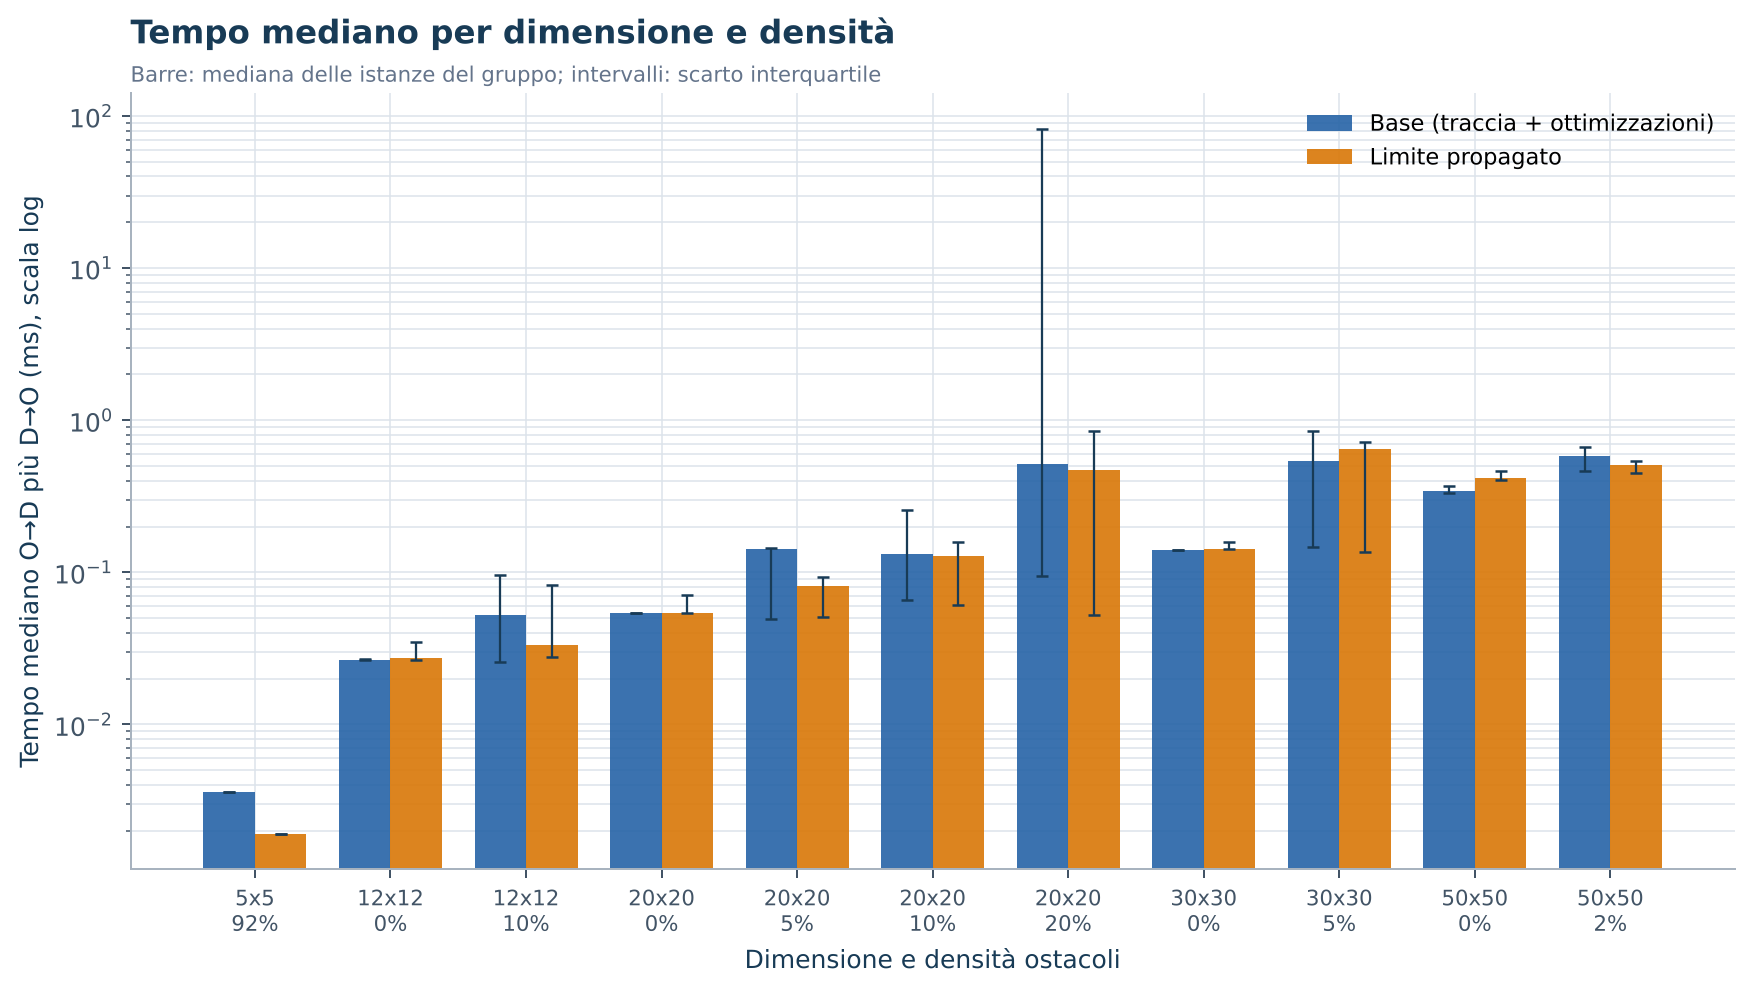
\includegraphics[width=0.92\textwidth]{grafico2_tempo_per_scenario.png}
  \caption{Tempo mediano $O \to D$ più $D \to O$ per dimensione e densità,
  varianti \code{base} e \code{limite-propagato} (scala logaritmica). Le
  barre d'errore sono l'intervallo interquartile delle istanze del gruppo.}
  \label{fig:tempo-scenario}
\end{figure}

Dalla tabella e dalla \cref{fig:tempo-scenario} emergono tre aspetti.

\begin{itemize}
  \item \textbf{Senza ostacoli il tempo cresce con la dimensione.} In tutte
        le 12 istanze senza ostacoli $D$ è nella chiusura di $O$ e basta una
        chiamata per verso. Il tempo della variante \code{base} sale da
        \num{0.027} ms a $12\times12$ a \num{0.34} ms a $50\times50$: le
        celle aumentano di 17 volte e il tempo di 13, come atteso da un
        calcolo di chiusura di costo $\Theta(n)$. Il passaggio di
        riscaldamento evita che la prima griglia misurata risulti più lenta
        di griglie più grandi a causa della compilazione JIT.
  \item \textbf{Il costo dipende dalle chiamate più che dalla dimensione.}
        Il gruppo più costoso per la variante \code{base} non è il
        $50\times50$ ma il $20\times20$ con il 20\% di ostacoli, dove una
        singola istanza richiede \num{102202} chiamate e \num{399} ms, circa
        due terzi del tempo della variante \code{base} sull'intero piano. Le
        istanze di uno stesso gruppo differiscono fino a quattro ordini di
        grandezza, perché la disposizione degli ostacoli e la posizione di
        $O$ e $D$ decidono quanti rami sopravvivono alla potatura.
  \item \textbf{Il limite propagato elimina le code.} Le mediane delle due
        varianti sono simili, perché la maggior parte delle istanze è facile
        per entrambe; il massimo del gruppo $20\times20$ al 20\% scende però
        da \num{399} ms a \num{2.1} ms e da \num{102202} a 719 chiamate.
\end{itemize}

\begin{figure}[H]
  \centering
  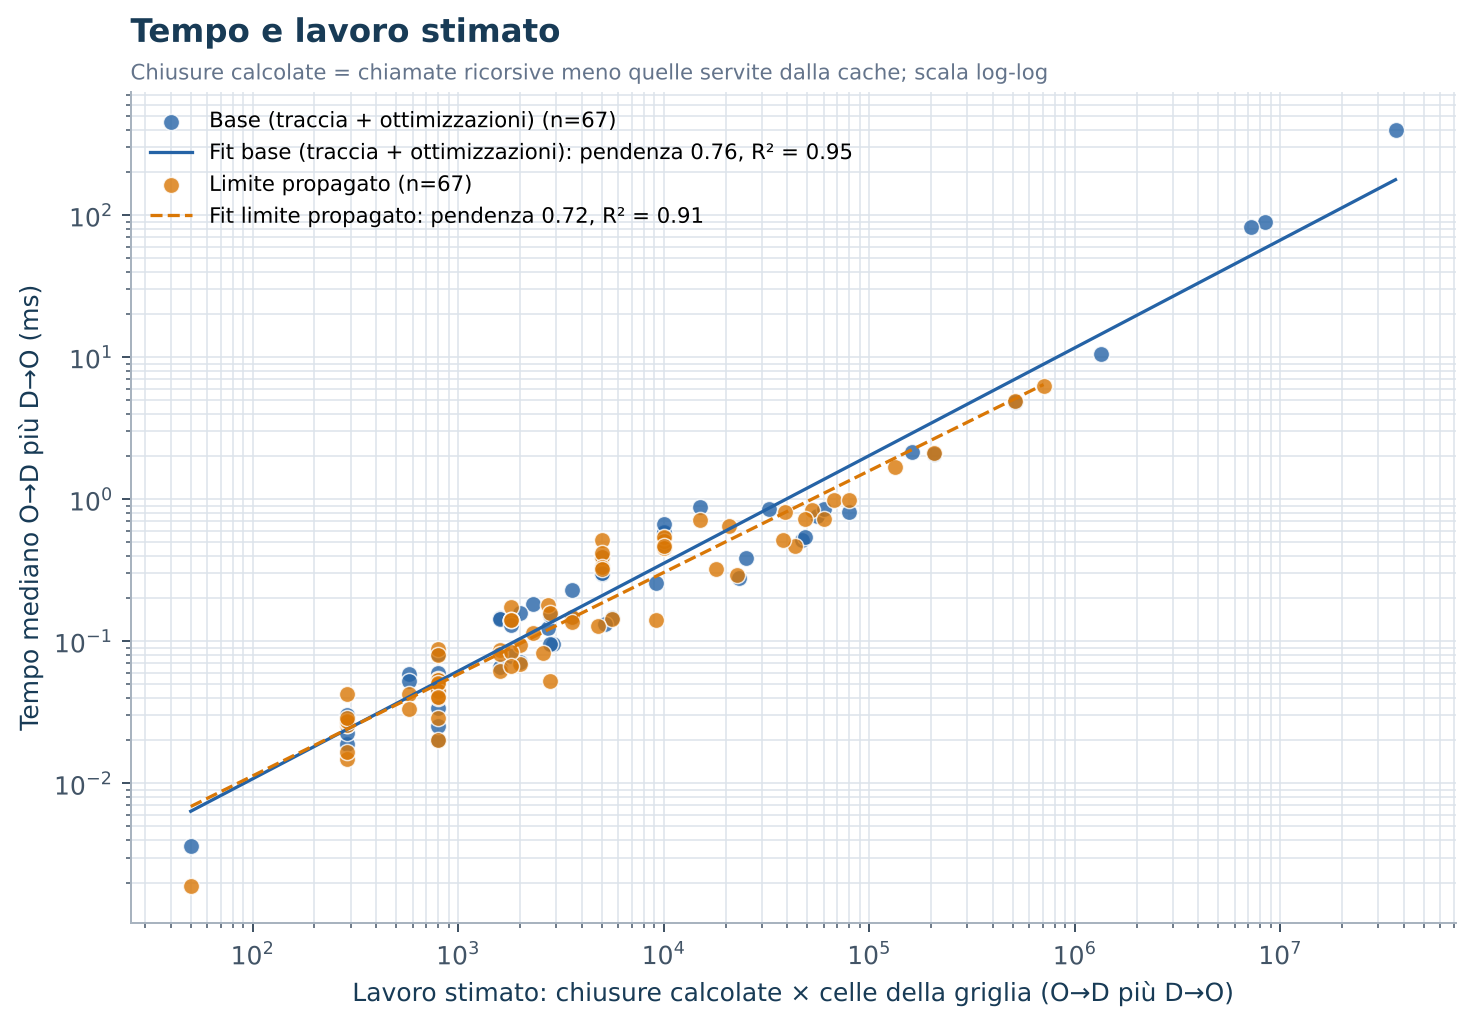
\includegraphics[width=0.82\textwidth]{grafico1_lavoro_vs_tempo.png}
  \caption{Tempo mediano rispetto al lavoro stimato $C_c \cdot n$ per le 67
  istanze, varianti \code{base} e \code{limite-propagato}, in scala log-log,
  con le rette di regressione.}
  \label{fig:lavoro-tempo}
\end{figure}

\paragraph{Che cosa determina il tempo.} La \cref{tab:predittori} confronta
quattro grandezze come predittori del tempo della variante \code{base}. Il
numero di chiamate da solo spiega il tempo in modo moderato, perché le
chiamate servite dalla cache costano poco e perché lo stesso numero di
chiusure costa di più su una griglia più grande. Il lavoro stimato
$C_c \cdot n$ della \cref{eq:tempo}, cioè le chiusure effettivamente
calcolate moltiplicate per le celle, spiega invece il 95\% della varianza
dei logaritmi (\cref{fig:lavoro-tempo}); la relazione vale anche per il
limite propagato ($R^2 = \num{0.909}$, $\rho = \num{0.955}$). La pendenza
minore di 1 indica che sulle istanze più piccole pesano costi fissi, come
l'allocazione dei risultati e le misure stesse, che non crescono con il
lavoro.

\begin{table}[H]
\centering
\small
\begin{tabular}{@{}l r r r r@{}}
\toprule
\textbf{Predittore} & \textbf{Istanze} & \textbf{Spearman $\rho$} & \textbf{Pendenza log-log} & $\mathbf{R^2}$ \\
\midrule
chiamate ricorsive $C$             & 67 & \num{0.737} & \num{0.704} & \num{0.753} \\
chiusure calcolate $C_c$           & 67 & \num{0.740} & \num{0.737} & \num{0.767} \\
celle di frontiera visitate        & 54 & \num{0.905} & \num{1.260} & \num{0.901} \\
lavoro stimato $C_c \cdot n$       & 67 & \num{0.957} & \num{0.759} & \num{0.953} \\
\bottomrule
\end{tabular}
\caption{Grandezze che spiegano il tempo mediano della variante \code{base};
per la frontiera si escludono le 13 istanze in cui è vuota. Le tre coppie di
una stessa griglia non sono osservazioni indipendenti: i valori descrivono
il piano e non permettono inferenze generali.}
\label{tab:predittori}
\end{table}

\paragraph{Potatura.} Sull'intero piano, con la variante \code{base}, la
condizione della riga 16 è risultata falsa \num{3423} volte; in altri
\num{20483} casi la riga 16 era vera e il ramo è stato potato dalla
condizione più forte della riga 17. Il dato descrive l'esecuzione con
entrambe le condizioni attive e non equivale al confronto fra le due
condizioni, che richiederebbe di eseguire l'algoritmo con la sola riga 16.

\begin{figure}[H]
  \centering
  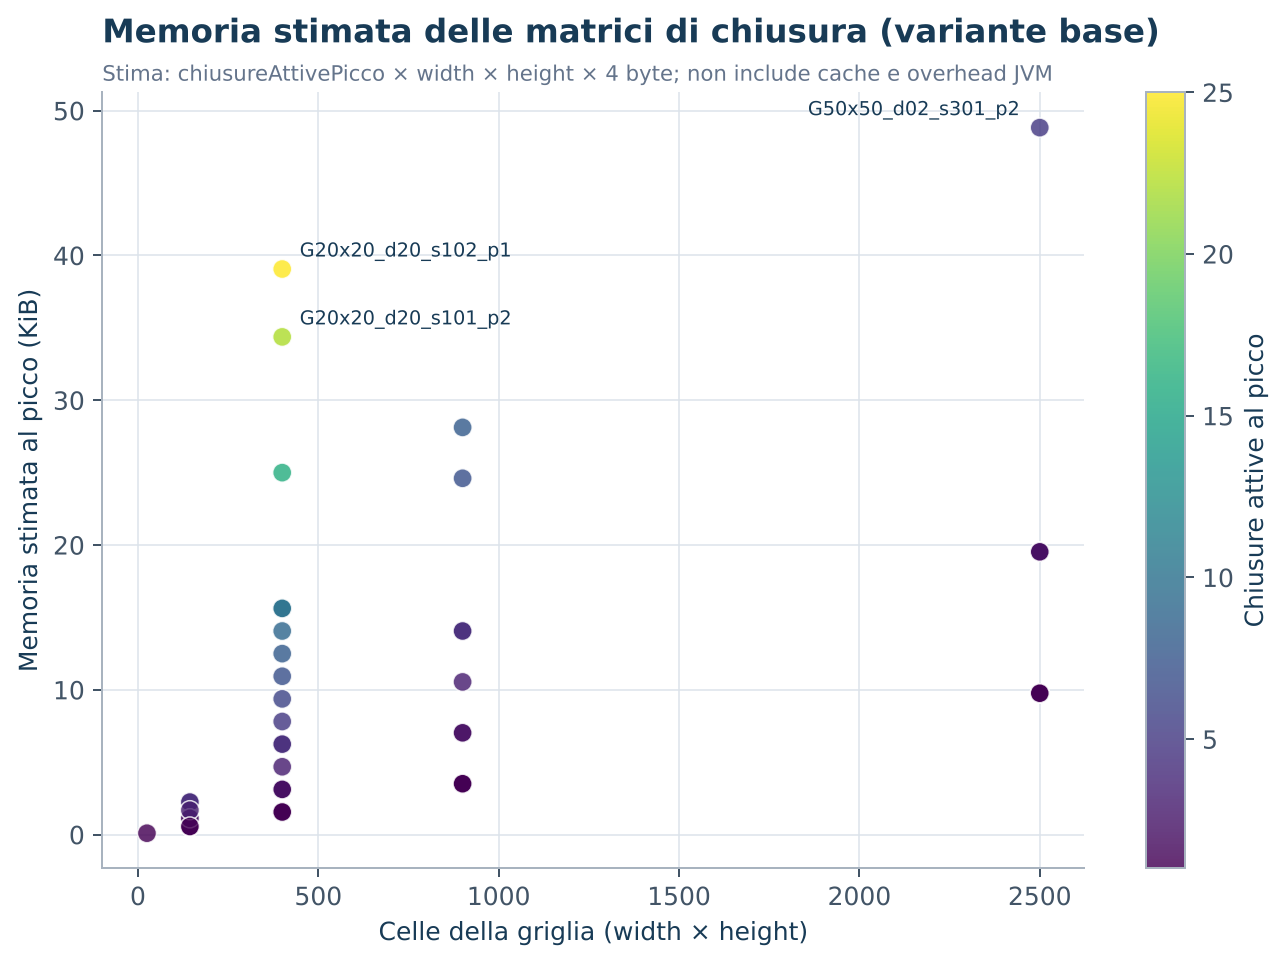
\includegraphics[width=0.75\textwidth]{grafico5_memoria_e_profondita.png}
  \caption{Memoria stimata delle matrici di chiusura attive
  contemporaneamente, variante \code{base}, rispetto al numero di celle; il
  colore indica il numero di matrici.}
  \label{fig:memoria}
\end{figure}

\paragraph{Memoria.} La memoria stimata delle matrici di chiusura
(\cref{fig:memoria}) non supera mai \num{50000} byte: il massimo corrisponde a
cinque matrici della griglia $50\times50$. Nell'istanza $20\times20$ più
costosa la ricorsione raggiunge profondità 25 con 25 matrici attive
insieme, cioè $25 \cdot 400 \cdot 4 = \num{40000}$ byte. Come osservato nella
\cref{sec:analisi-teorica}, la stima non comprende la cache.

\subsection{Effetto delle ottimizzazioni}
\label{sec:ablation}

La \cref{tab:ablation} e la \cref{fig:ablation} confrontano le quattro
varianti sui gruppi del piano con ostacoli. Per ogni gruppo sono riportati
il numero totale di chiamate ricorsive e la somma dei tempi mediani delle
istanze.

\begin{table}[H]
\centering
\small
\setlength{\tabcolsep}{4.2pt}
\begin{tabular}{@{}l r r r r r r r r@{}}
\toprule
& \multicolumn{2}{c}{\textbf{base}} & \multicolumn{2}{c}{\textbf{senza-cache}} &
  \multicolumn{2}{c}{\textbf{senza-ordinamento}} & \multicolumn{2}{c}{\textbf{limite-propagato}} \\
\cmidrule(lr){2-3}\cmidrule(lr){4-5}\cmidrule(lr){6-7}\cmidrule(l){8-9}
\textbf{Gruppo} & \textbf{chiamate} & \textbf{ms} & \textbf{chiamate} & \textbf{ms} &
  \textbf{chiamate} & \textbf{ms} & \textbf{chiamate} & \textbf{ms} \\
\midrule
$12\times12$, 10,4\% & 93            & \num{0.6}   & 97            & \num{0.8}    & 339        & \num{1.4}  & 88         & \num{0.5}  \\
$20\times20$, 5\%    & 189           & \num{1.6}   & 430           & \num{2.6}    & 941        & \num{5.6}  & 145        & \num{1.4}  \\
$20\times20$, 10\%   & 680           & \num{3.3}   & \num{1008}    & \num{5.0}    & \num{8397} & \num{30.1} & 365        & \num{2.0}  \\
$20\times20$, 20\%   & \num{149515}  & \num{574.7} & \num{608608}  & \num{2542.4} & ---        & ---        & \num{1608} & \num{6.0}  \\
$30\times30$, 5\%    & \num{1457}    & \num{8.5}   & \num{8707}    & \num{66.1}   & ---        & ---        & \num{1444} & \num{8.4}  \\
$50\times50$, 2\%    & 588           & \num{14.7}  & 588           & \num{14.0}   & ---        & ---        & 312        & \num{10.1} \\
\bottomrule
\end{tabular}
\caption{Chiamate ricorsive totali e somma dei tempi mediani per gruppo e
variante; --- indica una variante non eseguita nel gruppo.}
\label{tab:ablation}
\end{table}

\begin{figure}[H]
  \centering
  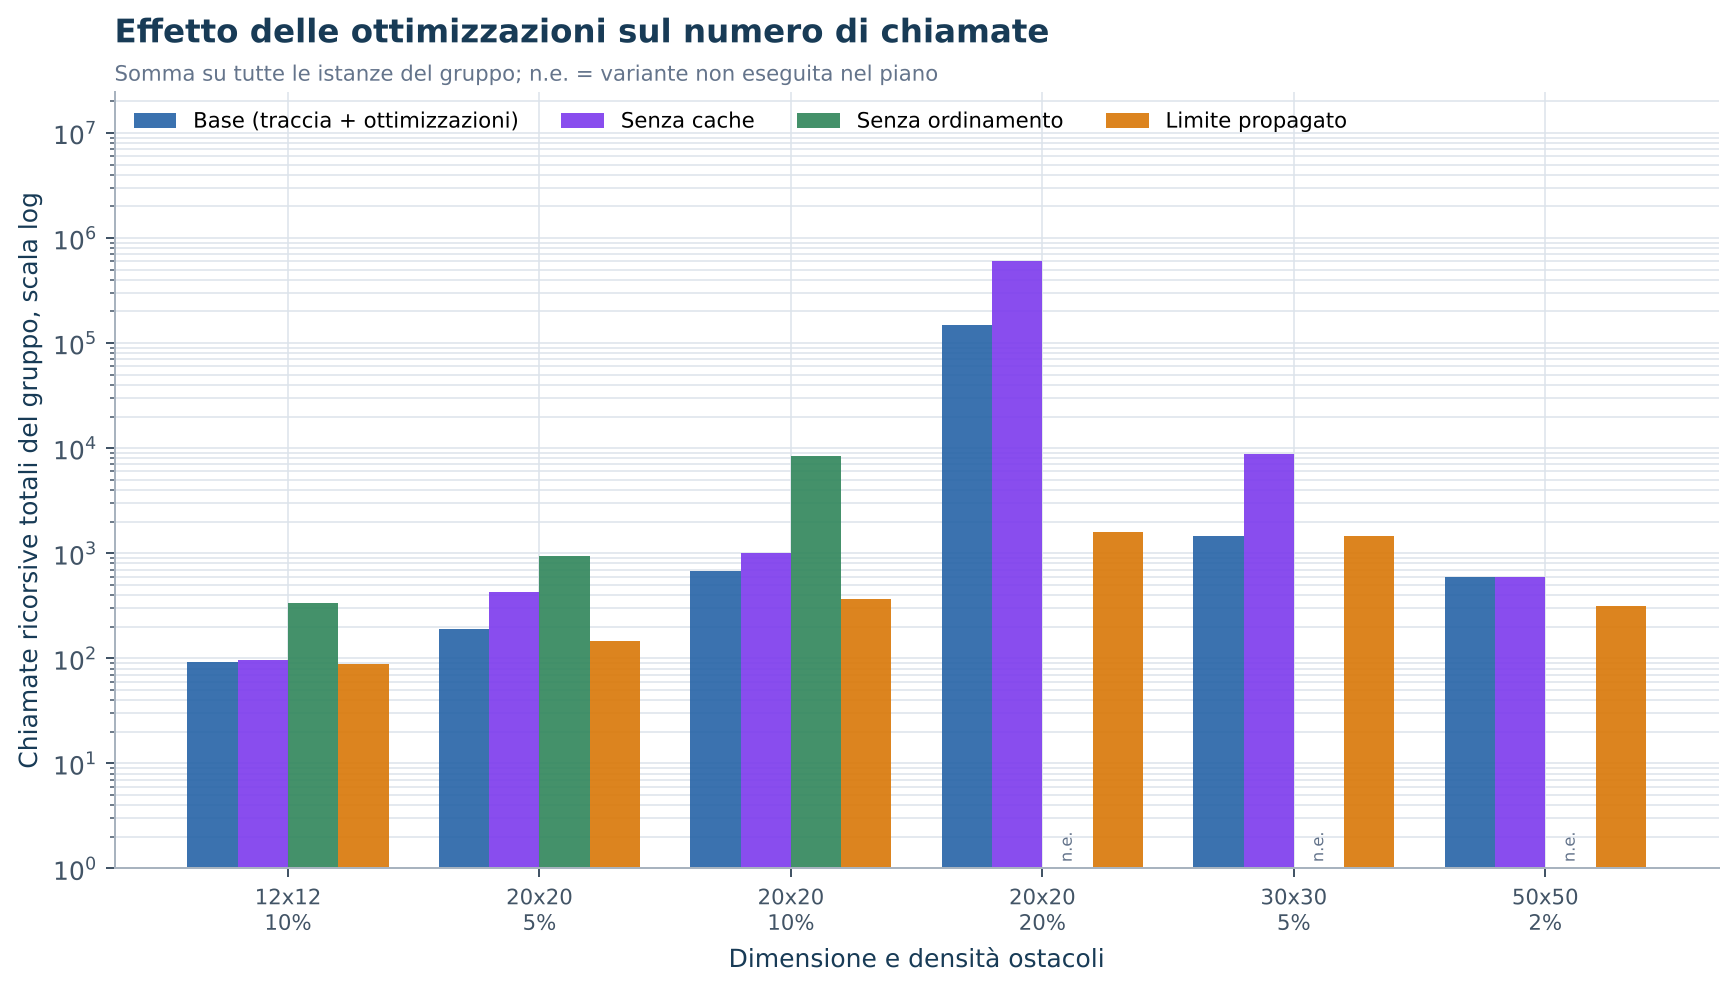
\includegraphics[width=0.92\textwidth]{grafico3_ablation.png}
  \caption{Chiamate ricorsive totali per gruppo e variante, in scala
  logaritmica.}
  \label{fig:ablation}
\end{figure}

\begin{itemize}
  \item \textbf{Ordinamento della frontiera.} È l'ottimizzazione più
        importante fra quelle della versione \code{base}: senza ordinamento le
        chiamate aumentano da 3,6 a 12 volte già sulle griglie più facili, e
        sulle griglie $20\times20$ al 20\% l'esecuzione diventa
        impraticabile. Visitando prima i candidati con limite inferiore
        minore, $\mathit{lunghezzaMin}$ scende subito e le righe 16 e 17
        potano quasi tutti gli altri rami.
  \item \textbf{Cache.} Il guadagno cresce con la difficoltà: senza cache le
        chiamate sono 4 volte tante a $20\times20$ al 20\% e 6 volte tante a
        $30\times30$ al 5\%, con tempi 4,4 e 7,8 volte maggiori. Sulle
        griglie $50\times50$ al 2\% non ci sono sottoproblemi ripetuti e la
        cache non cambia nulla.
  \item \textbf{Limite propagato.} Sull'intero piano riduce le chiamate da
        \num{152548} a \num{3988}; nel gruppo $20\times20$ al 20\% le riduce
        di 93 volte e il tempo di 96 volte. Sui gruppi in cui la versione
        \code{base} trova subito il cammino migliore il guadagno è piccolo o
        nullo, come a $30\times30$ al 5\%.
\end{itemize}

\subsection{Limiti di scala}
\label{sec:limiti-scala}

Il piano principale arriva a $50\times50$ con il 2\% di ostacoli. Per capire
dove l'algoritmo smette di essere utilizzabile, la classe \code{LimitiScala}
esegue una serie separata, salvata in \code{risultati/limiti\_scala.csv},
per le varianti \code{base} e \code{limite-propagato}:

\begin{itemize}
  \item griglie quadrate di lato 20, 30, 40, 50, 70 e 100;
  \item densità di ostacoli 0, 5, 10, 15, 20 e 30\%;
  \item tre seed (1, 2, 3) per combinazione, per un totale di 108 coppie per
        variante;
  \item $O$ nella cella libera più vicina al 10\% della diagonale e $D$ in
        quella più vicina al 90\%;
  \item ogni verso eseguito in una JVM separata con limite di \textbf{10 s}
        e memoria massima di \textbf{1 GB}; $D \to O$ viene eseguito solo se
        $O \to D$ è terminato.
\end{itemize}

Il processo separato permette di registrare un superamento del limite di
tempo (\code{TIMEOUT}) o un \code{OutOfMemoryError} (\code{OOM}) e passare
alla coppia successiva senza aggiungere a \cmin{} un meccanismo di
interruzione, che per questa versione non è richiesto. Ogni verso è una
singola esecuzione senza riscaldamento: i tempi comprendono l'avvio della
JVM e la compilazione JIT e non sono confrontabili con quelli del piano. La
serie è stata eseguita l'8 novembre 2026 sulla stessa macchina del piano, in
circa 18 minuti.

\begin{table}[H]
\centering
\small
\begin{tabular}{@{}l c c c c c c@{}}
\toprule
\textbf{Dimensione} & \textbf{0\%} & \textbf{5\%} & \textbf{10\%} & \textbf{15\%} & \textbf{20\%} & \textbf{30\%} \\
\midrule
$20\times20$   & 3 \;|\; 3 & 3 \;|\; 3 & 3 \;|\; 3 & 3 \;|\; 3 & 3 \;|\; 3 & 3 \;|\; 3 \\
$30\times30$   & 3 \;|\; 3 & 3 \;|\; 3 & 2 \;|\; 3 & 1 \;|\; 3 & 0 \;|\; 3 & 0 \;|\; 3 \\
$40\times40$   & 3 \;|\; 3 & 3 \;|\; 3 & 1 \;|\; 3 & 0 \;|\; 0 & 0 \;|\; 2 & 0 \;|\; 2 \\
$50\times50$   & 3 \;|\; 3 & 2 \;|\; 2 & 0 \;|\; 2 & 0 \;|\; 2 & 0 \;|\; 1 & 0 \;|\; 1 \\
$70\times70$   & 3 \;|\; 3 & 0 \;|\; 1 & 0 \;|\; 3 & 0 \;|\; 0 & 0 \;|\; 1 & 0 \;|\; 0 \\
$100\times100$ & 3 \;|\; 3 & 1 \;|\; 2 & 0 \;|\; 0 & 0 \;|\; 0 & 0 \;|\; 0 & 0 \;|\; 0 \\
\midrule
\textbf{Totale} & \multicolumn{6}{c}{\textbf{46} su 108 \;|\; \textbf{73} su 108} \\
\bottomrule
\end{tabular}
\caption{Coppie completate in entrambi i versi entro i limiti, su 3 per
cella: \code{base} a sinistra, \code{limite-propagato} a destra.}
\label{tab:limiti}
\end{table}

\begin{figure}[H]
  \centering
  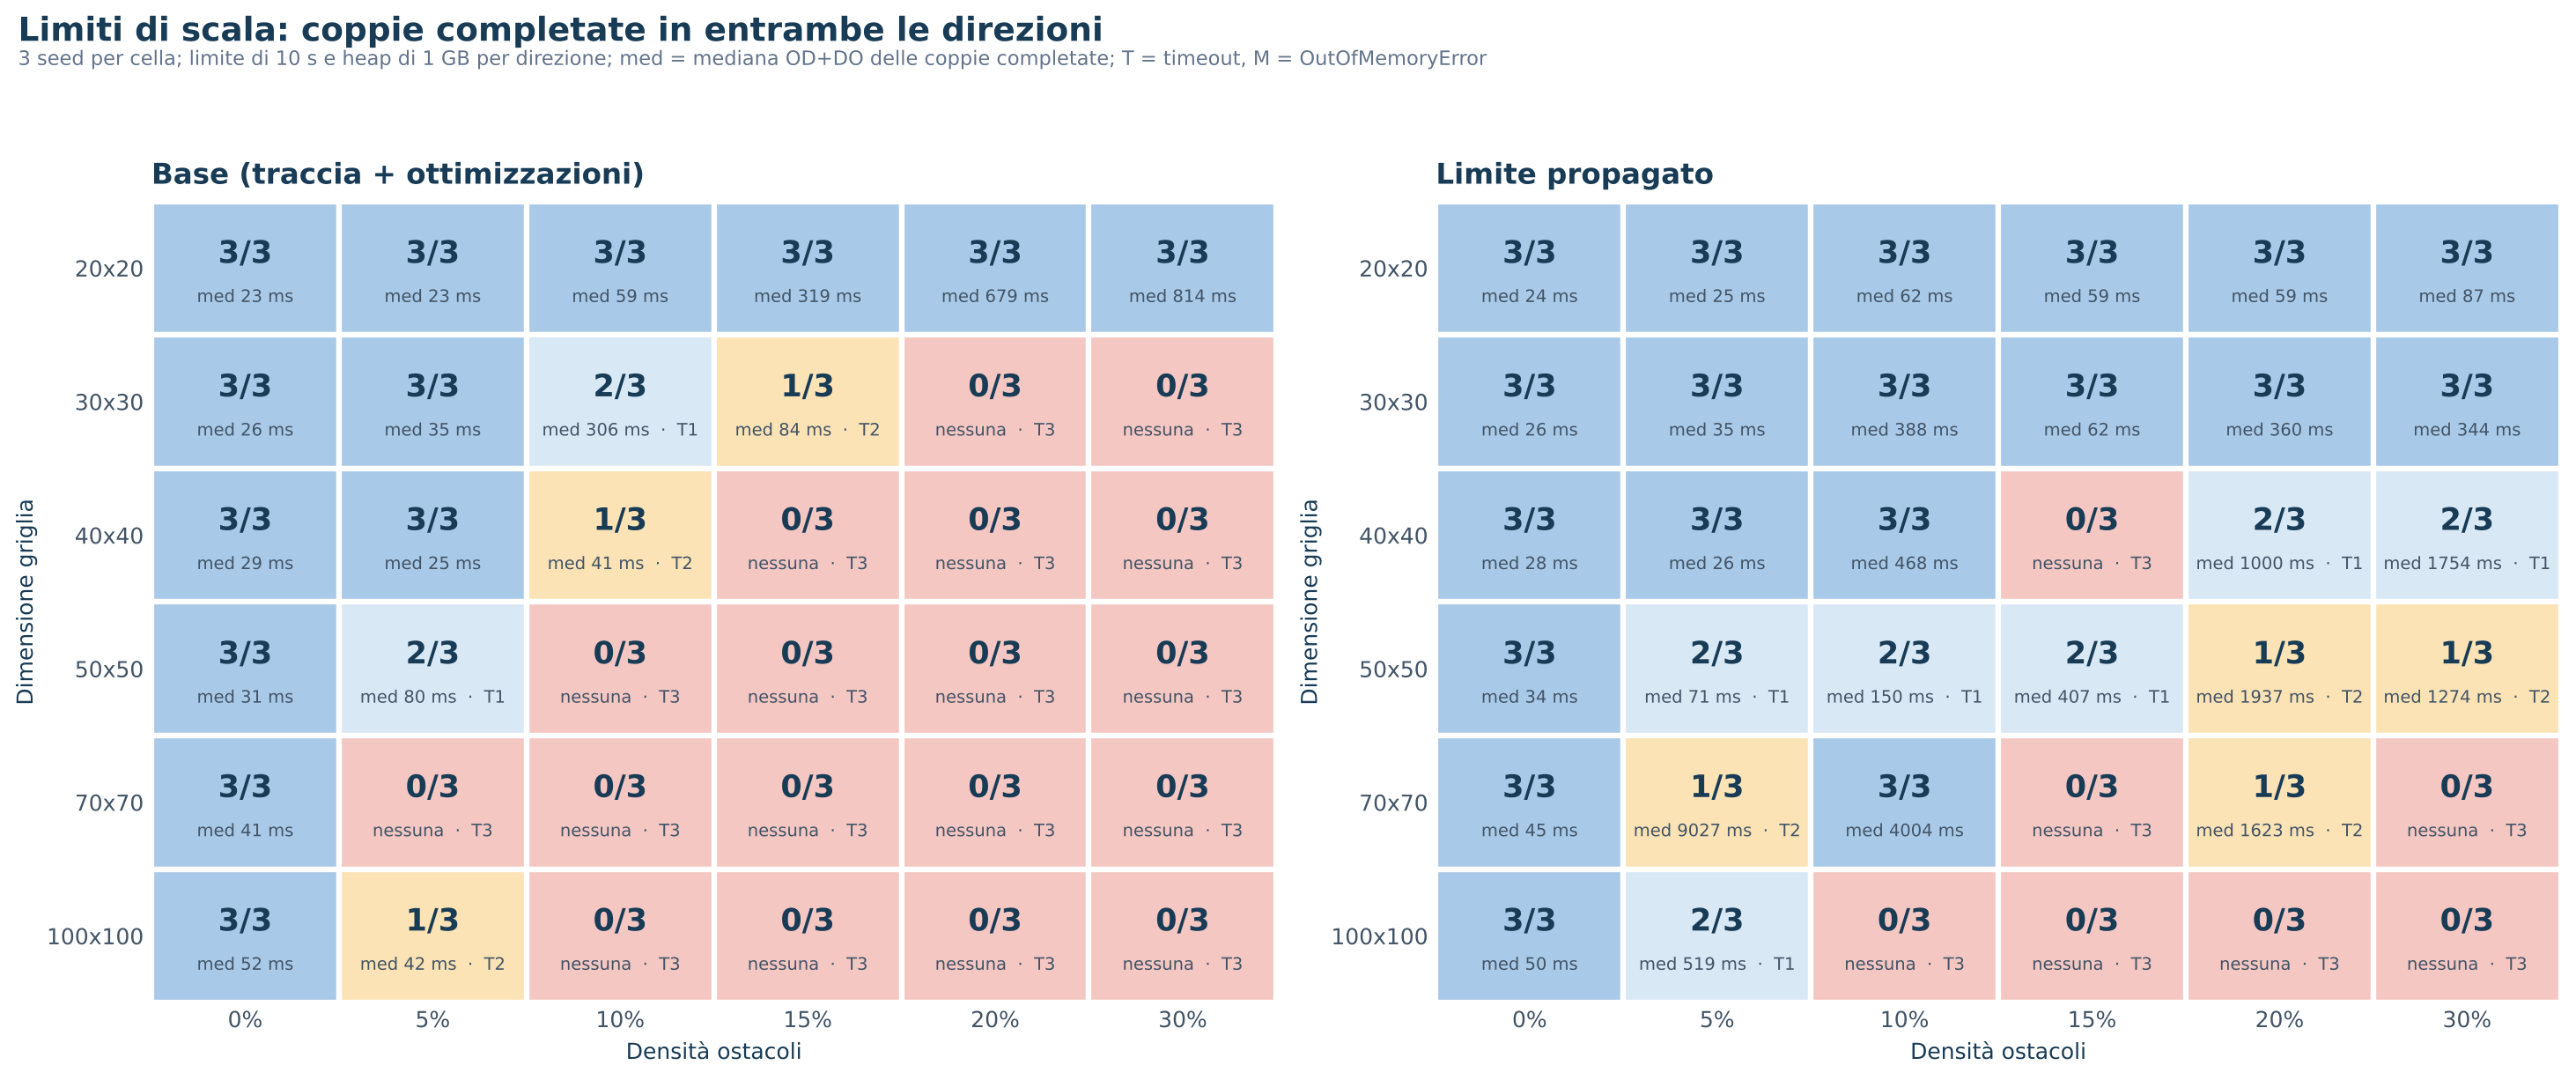
\includegraphics[width=\textwidth]{grafico6_limiti_scala.png}
  \caption{Esito della serie sui limiti di scala per le due varianti. In ogni
  cella: coppie completate, mediana del tempo $O \to D$ più $D \to O$ delle
  coppie completate e numero di esecuzioni fermate per tempo (T) o per
  memoria (M).}
  \label{fig:limiti}
\end{figure}

Con la variante \code{base} sono state completate 46 coppie su 108: le altre
62 si sono fermate per il limite di tempo già nel verso $O \to D$. Con il
limite propagato le coppie completate sono 73: le stesse 46 più altre 27,
mentre 34 si sono fermate nel verso $O \to D$ e una nel verso $D \to O$,
sempre per il limite di tempo. Nessuna esecuzione ha esaurito la memoria.
Tutte le coppie completate sono simmetriche e, dove entrambe le varianti
terminano, le lunghezze coincidono. Numero di chiamate e lunghezze non
dipendono dalla macchina; su hardware diverso possono cambiare esito solo le
coppie che terminano vicino ai 10 s.

Dalla serie emergono cinque osservazioni.

\begin{enumerate}
  \item \textbf{Senza ostacoli la dimensione non è un problema.} Le 18 coppie
        allo 0\% terminano con una sola chiamata per verso, perché in assenza
        di ostacoli ogni cella della griglia appartiene al contesto di $O$. I
        tempi, fra 23 e 52 ms anche a $100\times100$, sono quelli di un
        calcolo di chiusura con la JVM appena avviata.
  \item \textbf{Per la variante \code{base} il fattore critico è la
        densità.} A $20\times20$ tutte le densità sono gestibili, ma la
        mediana passa da 23 ms allo 0\% a 814 ms al 30\%. A $30\times30$ si
        perdono coppie dal 10\% in su, a $50\times50$ resta parzialmente
        gestibile solo il 5\%, a $70\times70$ e $100\times100$ nessuna
        densità diversa da zero è gestibile in modo affidabile.
  \item \textbf{Il limite propagato sposta il confine.} Completa tutte le
        coppie $30\times30$ fino al 30\% e più della metà di quelle
        $40\times40$ e $50\times50$ con ostacoli. Sulle 46 coppie completate da entrambe le varianti,
        le chiamate del verso $O \to D$ scendono da \num{1096774} a
        \num{20140}. La coppia più costosa per la variante \code{base}
        ($20\times20$, 30\%, seed 1) richiede \num{480274} chiamate,
        profondità 24, \num{2.1} s e fino a 390 MB di heap; con il limite
        propagato bastano 362 chiamate, 49 ms e 9 MB.
  \item \textbf{La crescita resta combinatoria.} Anche con il limite
        propagato le griglie $70\times70$ e $100\times100$ superano quasi
        sempre i 10 s; la coppia completata più costosa ($70\times70$, 5\%,
        seed 2) richiede \num{508161} chiamate e \num{8.8} s nel solo verso
        $O \to D$. Come previsto dalla \cref{sec:analisi-teorica}, le
        ottimizzazioni riducono il numero di chiamate ma non il caso
        peggiore.
  \item \textbf{I due versi possono costare in modo molto diverso.} Per
        ciascuna variante, in 5 coppie completate un verso è più lento
        dell'altro di oltre 10 volte, per esempio \num{1410} ms contro 29 ms
        a $20\times20$ con il 15\% (seed 3, \code{base}). Una spiegazione
        plausibile è che in un verso si trovi presto un cammino corto, che
        consente di potare molti più rami.
\end{enumerate}
